However before proving Montel's Big Theorem, we need the following important result.
\begin{lemma}[Zalcman's Lemma]\label{lem:zalcman}
    A family of meromorphic functions $\scrS$ on a domain $\Omega$ is \textit{not} normal in the chordal metric if and only if there exists a sequence $a_n \to a_{0} \in \Omega$, a sequence of positive numbers $\rho_n \to 0$ and a sequence function $f_n \in \scrS$ such that $g_n(z) = f_n(a_n + \rho_n z)$ converges uniformly on compact sets (in the chordal metric) to a \textit{non-constant} function $g(z)$. This function $g(z)$ is meromorphic on all of $\C$ and is such that $g^\#(z) \leq 1$ for all $z$ and $g^\#(0) = 1$.
\end{lemma}

The statement seems like a strange one initially because we check for normality by finding a convergent limit. In fact the non-normality condition is exactly related to the non-constant condition of $g$. It is useful to consider an example where we apply the lemma.
\begin{example}
    Suppose we have $\scrS = \{f_n\}$ where $f_n(z) = z^n$ which is normal on $D$ and $\C \setminus \ol{D}$ but not on any domain containing the unit circle (because any neighbourhood of a point on the unit circle will contain points that lie in the interior of the disk and the exterior. Points in the interior tend to 0 and points in the exterior tend to infinity, so we can't have normality). We can verify this using the lemma above. For example if we have $a_n = 1$ and $\rho_n = 1/n$. Then
    \begin{align*}
        f_n(a_n + \rho_n z) = \left(1 + \frac{z}{n}\right)^n \to e^z = g(z)
    \end{align*}
    Then notice that $g$ is meromorphic on all of $\C$ and 
    \begin{align*}
        g^\#(z) = \frac{2\abs{g'(z)}}{1 + \abs{g'(z)}^2} = \frac{2\abs{e^z}}{1 + \abs{e^z}^2} \leq 1
    \end{align*}
    and $g^\#(0) = 1$. 
\end{example}

\begin{proof}
    Suppose $\scrS$ is normal. Suppose we have any sequence $\{f_n\} \subset \scrS$ and by normality we can assume that the $f_n$ converge to $f$ (uniformly on compact subsets with respect to the chordal metric). Now take any sequence $a_n \to a_0 \in \Omega$ and positive real numbers $\rho_n \to 0$. Then we see that 
    \begin{align*}
        g_n(z) = f_n(a_n + \rho_n z) \to f(a_0)
    \end{align*}
    and hence is constant. This follows from the fact that the $f_n$ are equicontinuous (we know this from Arzelà–Ascoli). Therefore for any $\epsilon > 0$ there exists some $\delta$ such that if $\abs{a_n + \rho_n z - a_0} < \delta$ then $\abs{f_n(a_n + \rho_n z) - f_n(a_0)} < \epsilon$. Clearly for any $z$, we can find $n$ large enough so that $\abs{a_n + \rho_n z - a_0} < \delta$. But then if $z$ is on a compact set, we can make this choice for $n$ independently of $z$. Therefore $g_n$ converge to a constant function.
    % TODO: Verify details, need uniform equicontinuity?
    
    Now suppose $\scrS$ is not normal. We will construct the appropriate data from this. First, since $\scrS$ is not normal, we know that $\scrS^\#$ is not locally bounded so just as we did before we find $b_n \to b_0 \in \Omega$ and $f_n \in \scrS$ such that $f_n^\#(b_n) \to \infty$ as $n \to \infty$. By translating if necessary we can assume that $b_0 = 0$ and that $\Omega$ contains a closed disk of radius $r$ centered at 0. Then define
    \begin{align*}
        M_n &:= \sup_{\abs{\zeta} \leq r} (r - \abs{\zeta}) f_n^\#(\zeta)
    \end{align*}
    Since $\abs{\zeta} \leq r$ is a compact, we know the above sup is actually achieve so there is some $a_n$ in this closed disk such that 
    $$M_n = (r - \abs{a_n}) f_n^\#(a_n)$$
    We notice that $M_n \to \infty$ as $n \to \infty$ (since we know that $f_n^\#(b_n) \to \infty$). Now we take $\rho_n = 1/f_n^\#(a_n)$ and consider
    $$g_n(z) = f_n \left( a_n + \frac{z}{f_n^\#(a_n)} \right)$$
    which is defined on $\abs{z} \leq M_n$ since 
    \begin{align*}
        \abs{a_n + \frac{z}{f_n^\#(a_n)}} \leq \abs{a_n} +\frac{\abs{z}}{f_n^\#(a_n)} \leq \abs{a_n} +\frac{M_n}{f_n^\#(a_n)} = \abs{a_n} + r - \abs{a_n} = r
    \end{align*}

    Now fix $R < \infty$. Since $M_n \to \infty$, we know for sufficiently large $n$ we have $R < M_n$. Then for $\abs{z} \leq R$ we have 
    \begin{align}
        g_n^\#(z) &= \frac{f_n^\#(z_n + z/f_n^\#(a_n))}{f_n^\#(a_n)} \tag{``chain rule''}\\
        &\leq \frac{M_n}{r - \abs{a_n + z/f_n^\#(a_n)}} \cdot \frac{r - \abs{a_n}}{M_n} \tag{definition of $M_n$}\\
        &\leq \frac{r - \abs{a_n}}{r - \abs{a_n} - \abs{z_n}/f_n^\#(a_n)} \tag{Reverse triangle inequality}\\
        &= \frac{1}{1 - \abs{z}/M_n} \tag{factor out $r - \abs{a_n}$}
    \end{align}
    Then notice the last line converges to 1 as $n \to \infty$ (again since $M_n \to \infty$). Then by \hyperref[thm:marty]{Marty's Theorem} we know $\{g_n\}$ is a normal family so has a subsequence that converges uniformly on compact subsets in the chordal metric. Without loss of generality, we can assume this subsequence is $\{g_n\}$ itself and define $g := \lim_n g_n$. Notice by the above arguement that $g^\#(0) = 1$ and $g^\#(z) \leq 1$. Then $g$ is a meromorphic function and since $g^\#(0) \neq 0$, it is non-constant. Finally, we can have $a_n$ converging to $a_0 \in \Omega$ by passing to a subsequence (recall they form a sequence in the compact set $\abs{\zeta} \leq r$).
\end{proof}

\begin{theorem}[Montel's Big Theorem]\label{thm:montel-big-thm}
    A family $\scrS$ of meromorphic functions in a domain $\Omega$ which omit 3 given distinct values $a, b, c$ in $\C \cup \{\infty\}$  is normal in the chordal metric.
\end{theorem}
\begin{proof}
    First recall that we can check for normality on a domain by checking normality on all disks contained within the domain (see \autoref{lem:suitable-cover}). Therefore without loss of generality we can assume that $\Omega = D$. Moreover, by composing with a fractional linear transformation if necessary we can assume that the values omitted at $0, 1$ and $\infty$. Therefore $\scrS$ is a family on holomorphic functions on the disk $D$ that omits 0 and 1. Now define
    $$\scrS_m = \{f \in \Hom(D) : f \text{ omits } 0 \text{ and } e^{2\pi i k/2^m}, k = 0, \dots, 2^m - 1\}$$
    In other words $\scrS_m$ is the collection of holomorphic functions on the disk that miss the $2^m$-th roots of unity. Notice that $\scrS \subset \scrS_0$ so $\scrS_0$ is non-empty. Moreover every $f \in \scrS_m$ is non-vanishing so has a well-defined square root $f^{1/2}$ which is necessarily contained in $\scrS_{m + 1}$. Therefore no $\scrS_m$ is empty.

    Now suppose that $\scrS$ is not normal. Then there exists some $\{f_n\} \subset \scrS \subset \scrS_0$ that does not contain a convergent subsequence. Then $\{f_n^{1/2}\} \subset \scrS_1$ also has no convergent subsequence so $\scrS_1$ could not be normal. Continuing in this manner we conclude that none of the $\scrS_m$ are normal. Let $g_m$ be the corresponding ``$g$'' given by \hyperref[lem:zalcman]{Zalcman's Lemma} for each $\scrS_m$. Zalcman only guarantees that $g_m$ is meromorphic but by \autoref{cor:conv-holom-or-inf} we can conclude that $g_m$ must be holomorphic (and hence entire) as well. 
    
    We also know by Zalcman's lemma that $\abs{g_m^\#(z)} \leq 1$ for all $z$ and for all $m$. Therefore we can apply \hyperref[thm:marty]{Marty's Theorem} to conclude that the $g_m$ form a normal family. As usual then we can assume that the $g_m$ are convergent and let $g$ be the limit. Notice that $g$ is non-constant because $g^\#(0) = 1$ since each $g_m^\#(0) = 1$. Moreover, being the limit of the $g_m$ we must have that $g$ omits all the $2^m$ roots of unity. Then $g(\C)$ is either contained within the disk or contained in $\C \setminus \ol{D}$. In either case either $g$ is bounded or $1/g$ is bounded which would imply by Liouville that $g$ is constant, leading to a contradiciton.
\end{proof}

\begin{theorem}[Picard's Big Theorem]
    A meromorphic function in a punctured disk which omits 3 distinct values in $\C \cup \{\infty\}$ extends to a meromorphic function on the entire disk.
\end{theorem}
\begin{proof}
    As usual we can assume that the disk is centered at 0 and the values omitted are $0, 1$ and $\infty$. Let $\epsilon_n$ be a sequence of positive real numbers that strictly decrease to 0. Then consider $\scrS := \{f_n(z) := f(\epsilon_n z)\}$ which is a normal family on $\Omega := \{0 < \abs{z} < 2\}$ (we choose $\epsilon_n$ to be make this a valid domain) by \hyperref[thm:montel-big-thm]{Montel's Big Theorem}. Let $g$ be the limiting function. Since each $f(\epsilon_n z)$ is holomorphic, by the problem set we know that $g$ is either holomorphic on $\Omega$ or identically $\infty$. 
    
    Suppose $g$ is holomorphic on $\Omega$. Let $M$ be such that $\abs{g(z)} \leq M < \infty$ for $\abs{z} = 1$ which means that $\abs{f_n(z)} \leq M$ for $\abs{z} = \epsilon_n$. In fact by convergence, there is some $n_0$ such that for all $n \geq n_0$ we have $\abs{f_n(z)} \leq M + 1$ on $\abs{z} = \epsilon_n$. Therefore we can apply the maximum modulus principle (see \autoref{thm:max-mod-prin}) which roughly says that the modulus of a non-constant holomorphic function $f$ can only achieve a maximum on the boundary of its domain of definition. Considering $f_n$ restricted to the annulus $\epsilon_{n + 1} \leq \abs{z} \leq \epsilon_n$, we then conclude that $\abs{f_n(z)} \leq M + 1$ on this annulus (again for $n \geq n_0$). This means that $\abs{f(z)} \leq M + 1$ on $0 < \abs{z} \leq \epsilon_{n_0}$. Since $f$ is bounded in a neighbourhood of 0, we conclude that 0 is a removable singularity and hence $f$ extends to be holomorphic on the entire disk.
    
    On the other hand if $g$ is identically infinity, then we can apply the same argument to $1/f(\epsilon_n z)$ to conclude $1/f$ extends to be holomorphic at 0 and hence $f$ is meromorphic on the disk.
\end{proof}

\begin{theorem}[Picard's Little Theorem]
    Any non-constant entire function omits at most 1 value.
\end{theorem}
\begin{proof}
    An entire function either has a pole or an essential singularity at infinity. If we have a pole, then the function is a polynomial so we hit every value in $\C$. Otherwise we have an essential singularity at infinity and since $\C$ is a neighbourhood of this essential singularity, we know it's image can omit at most 1 value of $\C$.
\end{proof}

\section{Riemann Surfaces}\label{sec:riem-surf}

\subsection{Complex Manifolds}
A manifold with a complex structure of dimension $n$ is a Hausdorff topological space with a countable basis such that every point has a neighbourhood which is homeomorphic to an open subset of $\C^n$. Moreover, for any two so-called coordinate charts $(\varphi_i, U_i)$ and $(\varphi_j, U_j)$ we have that the map $\varphi_j \circ \varphi_i^{-1}: \varphi_i(U_i \cap U_j) \to \varphi_j(U_i \cap U_j)$ is holomorphic. We will mostly be interested in the case of $n = 1$. 

\begin{figure}[ht]
    \centering
    \includegraphics[scale=0.6]{Images/manifold_def.png}
    \caption{A manifold is covered by a collection of compatible charts}
    \label{fig:manifold-def}
\end{figure}

% TODO: Add diagram of manifold

\begin{example}[Riemann Sphere]
An important example of a manifold with a complex structure, and one we have already discussed in a fair bit of detail, is the Riemann sphere. In this case we can cover the entire sphere with 2 coordinate charts. Let $U = S^2 \setminus \{N\}$ and define
\begin{align*}
    \varphi_U: U \to \C\\
    (x, y, t) &\mapsto \frac{x + iy}{1 - t}
\end{align*} 
and $V := S^2 \setminus \{S\}$ with 
\begin{align*}
    \varphi_V: V \to \C\\
    (x, y, t) &\mapsto \frac{x - iy}{1 + t}
\end{align*}
Recall that the transition map $\varphi_{V} \circ \varphi_U^{-1}: \C \setminus \{0\} = \varphi_U(U \cap V) \to \varphi_V(U \cap V) = \C \setminus \{0\}$ is given by $z \mapsto 1/z$ which is certainly holomorphic on $\C \setminus \{0\}$. 
\end{example}

A map $f: M \to N$ between manifolds with complex structures is holomorphic if $\psi_j \circ f \circ \varphi_i^{-1}$ (defined on $\varphi_i(U_i \cap f^{-1}(V_j))$) are holomorphic for every $i$ and $j$, see \autoref{fig:holom-maps-mflds}.

\begin{figure}[ht]
    \centering
    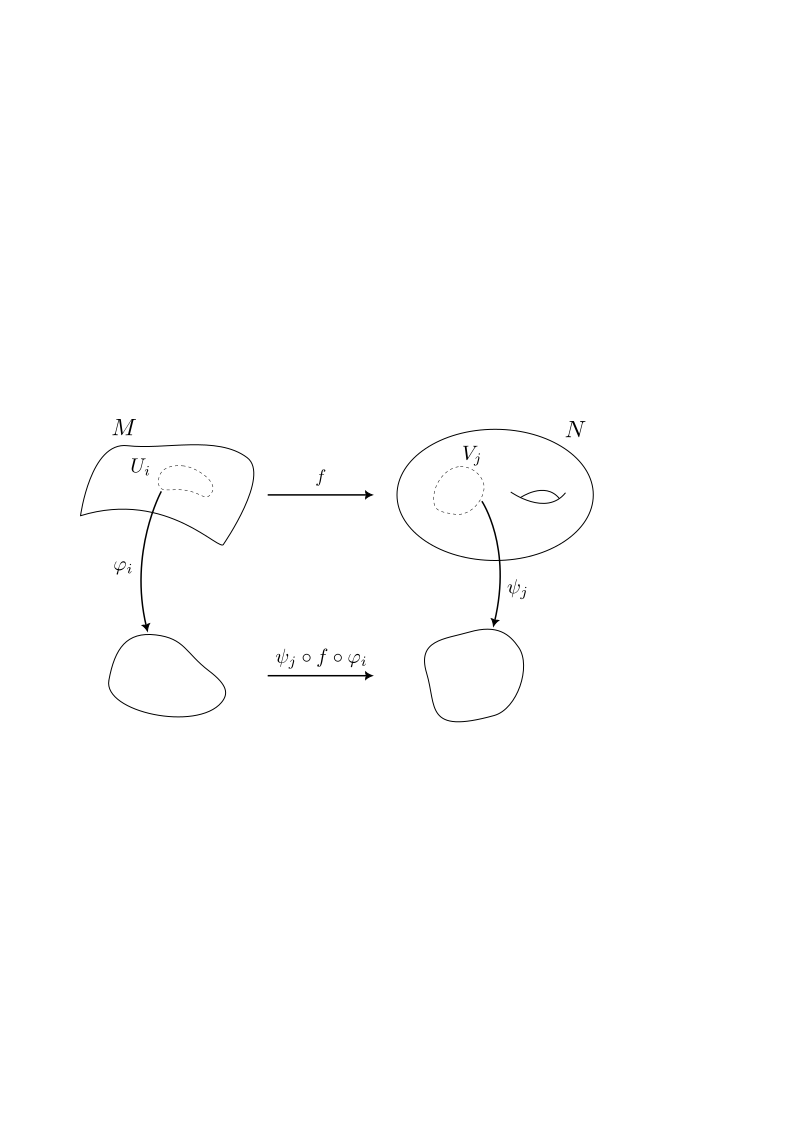
\includegraphics[scale=0.8]{Images/holom_maps_mflds.png}
    \caption{Map between manifolds with complex structure is holomorphic if it's holomorphic when viewed through charts}
    \label{fig:holom-maps-mflds}
\end{figure}

A holomorphic map $f: M \to N$ is an \textit{isomorphism} (or \textit{biholomorphism}) if it is a homeomorphism with a holomorphic inverse. We say two complex structures are equivalent if the identity map is a biholomorphism. Now we can finally given the proper definition of a complex manifold. 
\begin{definition}[Complex Manifold]
    A \textit{complex manifold} is a manifold with an equivalence class of complex structures.
\end{definition}
A complex manifold of dimension 1 is called a complex curve or more commonly a(n abstract) Riemann surface. 

The simplest examples of complex manifolds are of course $\C$ and $S^2$ or open subsets of them. A slightly more interesting example is $\C/\Z$ where we say that $z \sim z'$ if $z - z' \in \Z$. We can easily give this a complex structure. Let $p: \C \to \C/Z$ be the projection map on the quotient. Then for every $z_0 \in \C$, we can find an open neighbourhood $V$ of $z_0$ such that $p|_V$ is injective (for example we could take $V$ to be a disc of radius $1/2$). Then $p^{-1}$ acts as a coordinate chart on $p(V)$. 

Another example in a similar vein that we will explore more thoroughly is $\C/\Gamma$ where $\Gamma$ is a discrete subgroup of $\C$ (viewed as an additive group of course). Then we know that topologically $\C/\Gamma$ is a torus but different choices of $\Gamma$ may lead to torii with different complex structures (in particular $\C/\Gamma_1$ and $\C/\Gamma_2$ need not be biholomorphic). 

Importantly, the local properties of holomorphic functions holds for complex manifolds as well, practically by definition. Examples of such properties are the principle of analytic continuation, the maximum modulus principle, the mean value property, etc. A meromorphic function on a complex manifold $M$ is a holomorphic map from $M$ to $S^2$. For example, we have a 1-1 correspondence between meromorphic functions on $\C/\Gamma$ and meromorphic functions on $\C$ with $\Gamma$ as group of periods. 


